\documentclass[3pt,twocolumn]{elsarticle}
\usepackage[spanish]{babel}
\usepackage[utf8]{inputenc}
\usepackage[T1]{fontenc}
\usepackage{lineno,hyperref}
\modulolinenumbers[5]
\usepackage{graphicx}
\usepackage{subcaption}
\usepackage{listings}
\usepackage{ragged2e}
\usepackage{fontawesome}
%\lstset{style=mystyle}
\lstset{language=R, breaklines=true}
\usepackage{url}
\hypersetup{
    colorlinks=true,
    linkcolor=blue,
    filecolor=blue,      
    urlcolor=blue,
}
\usepackage{amsmath}
%\bibliographystyle{elsarticle-num}
%\captionsetup[subfigure]{labelformat=brace}

\makeatletter

\renewenvironment{abstract}{\global\setbox\absbox=\vbox\bgroup
  \hsize=\textwidth\def\baselinestretch{1}%
  \noindent\unskip\textbf{Resumen} 
 \par\medskip\noindent\unskip\ignorespaces}
 {\egroup}

\def\keyword{%
  \def\sep{\unskip, }%
 \def\MSC{\@ifnextchar[{\@MSC}{\@MSC[2000]}}
  \def\@MSC[##1]{\par\leavevmode\hbox {\it ##1~MSC:\space}}%
  \def\PACS{\par\leavevmode\hbox {\it PACS:\space}}%
  \def\JEL{\par\leavevmode\hbox {\it JEL:\space}}%
  \global\setbox\keybox=\vbox\bgroup\hsize=\textwidth
  \normalsize\normalfont\def\baselinestretch{1}
  \parskip\z@
  \noindent\textit{Palabras clave: }
  \raggedright                      
  \ignorespaces}

\def\ps@pprintTitle{%
     \let\@oddhead\@empty
     \let\@evenhead\@empty
     \def\@oddfoot{\footnotesize\itshape
        \ifx\@journal\@empty {Simulación computacional de nanomateriales}  
       \else\@journal\fi\hfill\today}%
     \let\@evenfoot\@oddfoot}
\usepackage{listings}
\usepackage{xcolor}

\definecolor{codegreen}{rgb}{0,0.6,0}
\definecolor{codegray}{rgb}{0.5,0.5,0.5}
\definecolor{codepurple}{rgb}{0.58,0,0.82}
\definecolor{backcolour}{rgb}{0.95,0.95,0.92}

\lstdefinestyle{mystyle}{
    backgroundcolor=\color{backcolour},   
    commentstyle=\color{codegreen},
    keywordstyle=\color{magenta},
    numberstyle=\tiny\color{codegray},
    stringstyle=\color{codepurple},
    basicstyle=\ttfamily\footnotesize,
    breakatwhitespace=false,         
    breaklines=true,                 
    captionpos=b,                    
    keepspaces=true,                 
    numbers=left,                    
    numbersep=5pt,                  
    showspaces=false,                
    showstringspaces=false,
    showtabs=false,                  
    tabsize=2
}

\lstset{style=mystyle}
%%%%%%%%%%%%%%%%%%%%%%%%%%%%%%%%%%%%%%%%%%%%%

\begin{document}

\twocolumn[
\begin{@twocolumnfalse}
\begin{frontmatter}
\title{Simulación del fenómeno de dispersión de electrones}
\author{{Rodríguez Regalado} N. D. \fnref{myfootnote}
\\ Correo electrónico: \href{mailto:nestor.rodriguezrgl@uanl.edu.mx}{nestor.rodriguezrgl@uanl.edu.mx \faEnvelope}
\\ \faGithub: 
\href{https://github.com/NestorZeus}{NestorZeus}
}
\address{Maestría en Ciencias de la Ingeniería con Orientación en Nanotecnología}

\address{Facultad de Ingeniería Mecánica y Eléctrica, Universidad Autónoma de Nuevo León}

\begin{abstract}
La dispersión de electrones es utilizada para estudiar la materia haciendo que un haz de electrones incida sobre una muestra. Cuando se forma el haz, el choque de partículas (electrones) con las moléculas del aire, se dispersan, y esto se debe a la reducida masa de los electrones. Los resultados obtenidos son extraídos calculando el porcentaje de la cantidad de electrones que lograron dispersarse fuera del centro del haz ya que el estar en el centro implica que son contados como haz directo y si dispersan fuera del centro son importantes para la información cristalográfica del material.
\end{abstract}

\begin{keyword}
Electrón \sep dispersión \sep átomo.
\end{keyword}
\end{frontmatter}
\end{@twocolumnfalse}
]

\section{Introducción}
En el campo de la nanotecnología existe un fenómeno importante para el estudio y la caracterización cristalográfica de los nanomateriales para una comprensión de la estructura y sus propiedades \cite{new_MC}, la interacción del electrón con los átomos de una muestra delgada se presenta en el microscopio electrónico de transmisión cuando se quiere analizar una muestra pequeña y estudiar la estructura cristalina para obtención de información cristalográfica. Cuando un haz de electrones es transmitido por la muestra existen interacciones como ionización, pérdida de energía, etc \cite{tem}. 

Una interacción importante característica del efecto en este microscopio es la fuerza eléctrica o interacción electrostática mejor conocido como fuerza de Coulomb que ocurre cuando un electrón que tiene carga negativa impacta contra un átomo (carga positiva) y su nube de electrones y ocasiona una atracción entre cada uno y a su vez una ligera repulsión, de esta manera dispersando el electrón en un ángulo dependiendo de la cercanía a la que pase del átomo. Estas dispersiones se utilizan como señales para obtener información cristalográfica de la muestra \cite{janecek2016modern}.

Comúnmente el análisis de \texttt{Monte Carlo} es utilizado para comprender este fenómeno en los microscopios y obtener una estimación de la dispersión dependiendo la muestra en el que analizan el efecto entre electrón-sólido \cite{new_MC}.

En el presente trabajo de simulación se diseña un modelo de dispersión de electrones con valor de carga $n$ que impacta a una muestra periódica de átomos correspondientes a muestras que se cambiaron para estudiar los distintos efectos de la dispersión debido a los tamaños de átomo y fuerzas de carga positiva de cada uno, obteniendo una estimación de electrones dispersados respecto a que tan cerca pasan del átomo. Como objetivos del trabajo se busca:
\begin{itemize}
    \item Generar el efecto de la interacción del electrón con átomo a una distancia mínima y replicar para una cantidad $n$ de electrones,
    \item variar la muestra de átomos simulando distintos elementos en el que cambia la carga positiva que repele al electrón y su tamaño para revisar el efecto que tiene en la dispersión,
    \item realizar un análisis estadístico de la cantidad de electrones dispersados y que tanto se alejaron del centro respecto a la cantidad de electrones y el tipo de material utilizado como muestra.
\end{itemize}
Este trabajo esta dividido primeramente hablando de los antecedentes de este tipo de simulaciones o estudios realizados donde principalmente se utiliza el método \texttt{Monte Carlo} para las estimaciones de la trayectoria del electrón, continuando con la sección de trabajos relacionados donde se revisa las simulaciones en las que se basa este código para realizar la implementación que en el capítulo de implementación de simulación se explica aunado a las herramientas utilizadas. Como final cuenta con las secciones de experimentos donde se habla del diseño de la simulación, los resultados obtenidos y una discusión de dichos resultados, terminando con una conclusión general del fenómeno simulado.

\section{Antecedentes}
En el siguiente articulo reportado se propone simular las trayectorias que siguen los electrones de un haz que incide en una muestra de un determinado material. Tomando un promedio de las dispersiones con modelos probabilısticos que son abordados con el método de Monte Carlo.

Estos efectos simulados son observados en la microscopıa electrónica la cual es una técnica de formación de imágenes basada en la incidencia de un haz de electrones sobre una muestra, donde ocurren los efectos por la fuerza de Coulomb ocasionada entre el haz de electrones y los átomos del material muestra. Surgen efectos de dispersión elástica la cual puede desencadenar simultáneamente la desviación de la trayectoria del electrón, debido a la atracción eléctrica y la velocidad de impacto del electrón.
Se describe que es complicado modelar para cada electrón los efectos que ocurren en el fenómeno, y se propone para solucionar esta tarea asignar probabilidades a ciertos eventos como que éste sea transmitido a través de la muestra a lo cual el método de Monte Carlo resulta eficiente \cite{saenzsimulacion}.
%%%%%%%%%%%%%%%%%%%%%%%%%%%%%%%%%%%%%%%%%%%%%%%%%%%%%%

En diversos trabajos se aborda el método Monte Carlo para resolver integrales o representar esta simulación de dispersión. 
Debido a que en los dominios de la física el método mencionado es popular para simular fenómenos descritos por la mecánica estadística como el transporte de neutrones reportado \cite{rubinstein2016simulation}.

%%%%%%%%%%%%%%%%%%%%%%%%%%%%%%%%%%%%%%%%%%%%%%%%%%%%%%
En otro trabajo similar utilizando el software \texttt{Python} producen haces de electrones paralelos dando condiciones de la velocidad de los electrones dado en kilovoltios y la desviación parabólica de cada uno dando un buen resultado a través de la simulación que se expone \cite{feng2017beam}.
%%%%%%%%%%%%%%%%%%%%%%%%%%%%%%%%%%%%%%%%%%%%%%%%%%%%%%

\subsection{Trabajos relacionados}
Esta simulación o implementación esta basada en dos trabajos, \href{https://satuelisa.github.io/simulation/p9.html}{Interacción entre partículas} y \href{https://satuelisa.github.io/simulation/p6.html}{Sistema multiagente} que pueden ser consultados en el repositorio de Schaeffer \cite{elisa}. Estas prácticas son seleccionadas ya que simulan un comportamiento similar al del electrón cuando sufre esta dispersión respecto a la distancia que se acerca al átomo.


\section{Modelo propuesto}
El modelo propuesto en el presente trabajo se basa en el fenómeno descrito por Cárter y Williams \cite{tem} en donde se explica la dispersión del electrón cuando impacta un átomo aislado para estudiar su efecto tal como se puede observar en la figura \ref{atomo} en como los electrones entre más cerca pasen del átomo sufrirán una mayor fuerza de atracción y por lo tanto el ángulo de dispersión sera mayor.  
\begin{figure}[h!]
    \centering
    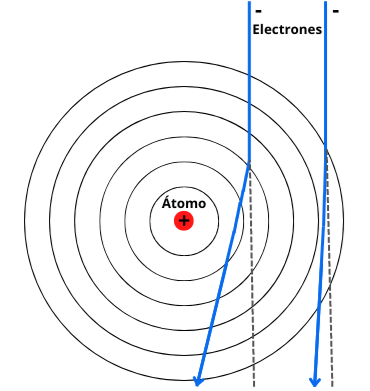
\includegraphics[scale=.65]{atomo.png}
    \caption{Interacción con átomo aislado.}
    \label{atomo}
\end{figure}
Ampliando el concepto del átomo aislado, de igual manera se plantea lo que sucede si los electrones impactan a un conjunto de átomos periódicamente distribuidos y lograr simular el efecto que ocurre en un material cristalino ya que cada dispersión representa una posición atómica de la muestra.

\section{Implementación de simulación}
El desarrollo de este código fue realizado en el lenguaje de programación \texttt{Python} \cite{Python}, así como librerías del mismo programa como \texttt{Numpy} \cite{numpy} y \texttt{Matplotlib} \cite{matplotlib} para la visualización de los gráficos y animaciones realizadas.

Partes importantes de la simulación del fenómeno se explican tal como puede ser visto código inicial \ref{code1} donde se declaran los electrones en sus posiciones al azar $(x,y)$ al igual que los átomos  solo que estos tendrán posiciones fijas.

\begin{lstlisting}[language=Python, caption=Declaración de electrones y átomos., label=code1]
electronX=[random.uniform(0,180) for i in range(n)]
electronY=[115 for i in range(n)]
planoX= [i for i in range(5,170,40)]
planoY= [80 for i in range(len(planoX))]
atomoP= [25 for i in range(len(planoX))]
\end{lstlisting}

Otra parte importante es donde cada electrón que se genera es comparada contra cada átomo obteniendo la distancia euclidiana y así de esta manera proceder en cada paso del electrón tal como se observa en el código \ref{code2}, dichas distancias son utilizadas para cuando el electrón entre en rango de la fuerza de atracción que se genera debido a las cargas opuestas entre electrón y átomo y de esta manera se genere un desvío en la trayectoria del electrón respecto a la distancia, si es muy cercano al átomo esta fuerza se incrementará.

\begin{lstlisting}[language=Python,caption=Distancia entre electron y átomo., label=code2] 
for xi, yi in electrones:
    A=[]
    electronY[cambioE]=electronY[cambioE]-paso
    for xf, yf in atomos: 
        distancia=sqrt(((xf-xi)**2)+((yf-yi)**2))
        if distancia <= Fuerza and yi>=yf:
            desvio=(pasomax/Fuerza)*(Fuerza-distancia)
\end{lstlisting}

Después de que el electrón entre en el rango de la fuerza de atracción del átomo se realiza una condición para que el electrón se desvié haciendo una probabilidad del cincuenta porciento, si se cumple esta condición entonces se realiza una comprobación de si la posición $x$ del electrón ($xi$) esta en el lado derecho del átomo entonces sufrirá una desviación negativa y viceversa para simular el efecto de atracción tal como se desarrolla en el código \ref{code3}. 
\begin{lstlisting}[language=Python,caption=Probabilidad y direccion del desvió., label=code3]
Pd=0.5
if (random.uniform(0,1))<Pd:
    if xi >= xf:
        electronX[cambioE]=electronX[cambioE]-desvio
        A.append('I')
    if xi < xf:
        electronX[cambioE]=electronX[cambioE]+desvio
        A.append('D')
\end{lstlisting}


\section{Experimentos}
La simulación desarrollada como primera instancia se simuló una secuencia de interacción de un electrón con un solo átomo para validar la dispersión del átomo aislado que puede ser visualizado en el repositorio de Rodríguez \cite{nestor}, en dicha simulación se puede observar como el electrón comienza a desviarse hasta el centro del átomo para cuando lo atraviesa cambia su dirección de dispersión debido a la interacción de coulomb que sufrió (ver figura \ref{atm_aislado}).
\begin{figure}[h!]
    \centering
    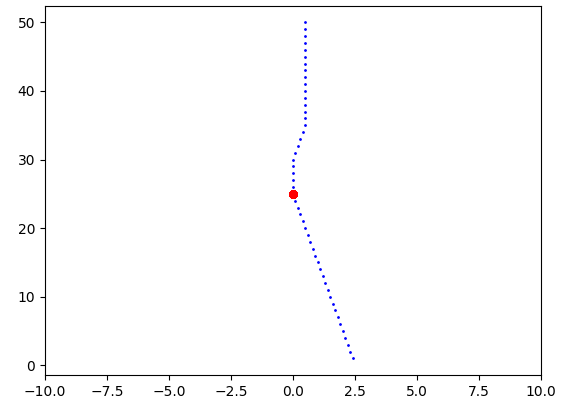
\includegraphics[scale=.4]{atm_elec.png}
    \caption{Electrón interacciona con átomo.}
    \label{atm_aislado}
\end{figure}
Este primer experimento del fenómeno descrito por Williams \cite{tem} fue ampliado a un concepto simulado en el que se logró colocar un conjunto de átomos y se procede a impactar una cantidad $n$ de electrones para estudiar la dispersión y entre más cerca del átomo se aproxime, mayor resulta la dispersión (ver figura \ref{5electrones}) y de misma manera se puede observar en el repositorio \cite{nestor}. 

\begin{figure}[h!]
    \centering
    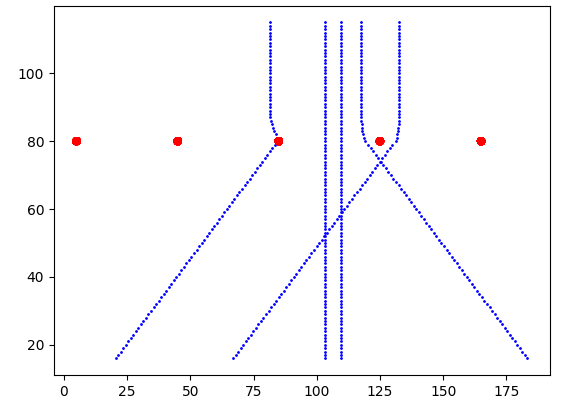
\includegraphics[scale=.4]{5electrones.png}
    \caption{Interaccion de conjunto de electrones con átomos.}
    \label{5electrones}
\end{figure}
\newpage
\subsection{Resultados}
Los resultados obtenidos son extraídos calculando el porcentaje de la cantidad de electrones que lograron dispersarse fuera del centro del haz ya que el estar en el centro implica que son contados como haz directo y si dispersan fuera del centro son importantes para la información cristalográfica del material.

\begin{figure}[h!]
    \centering
    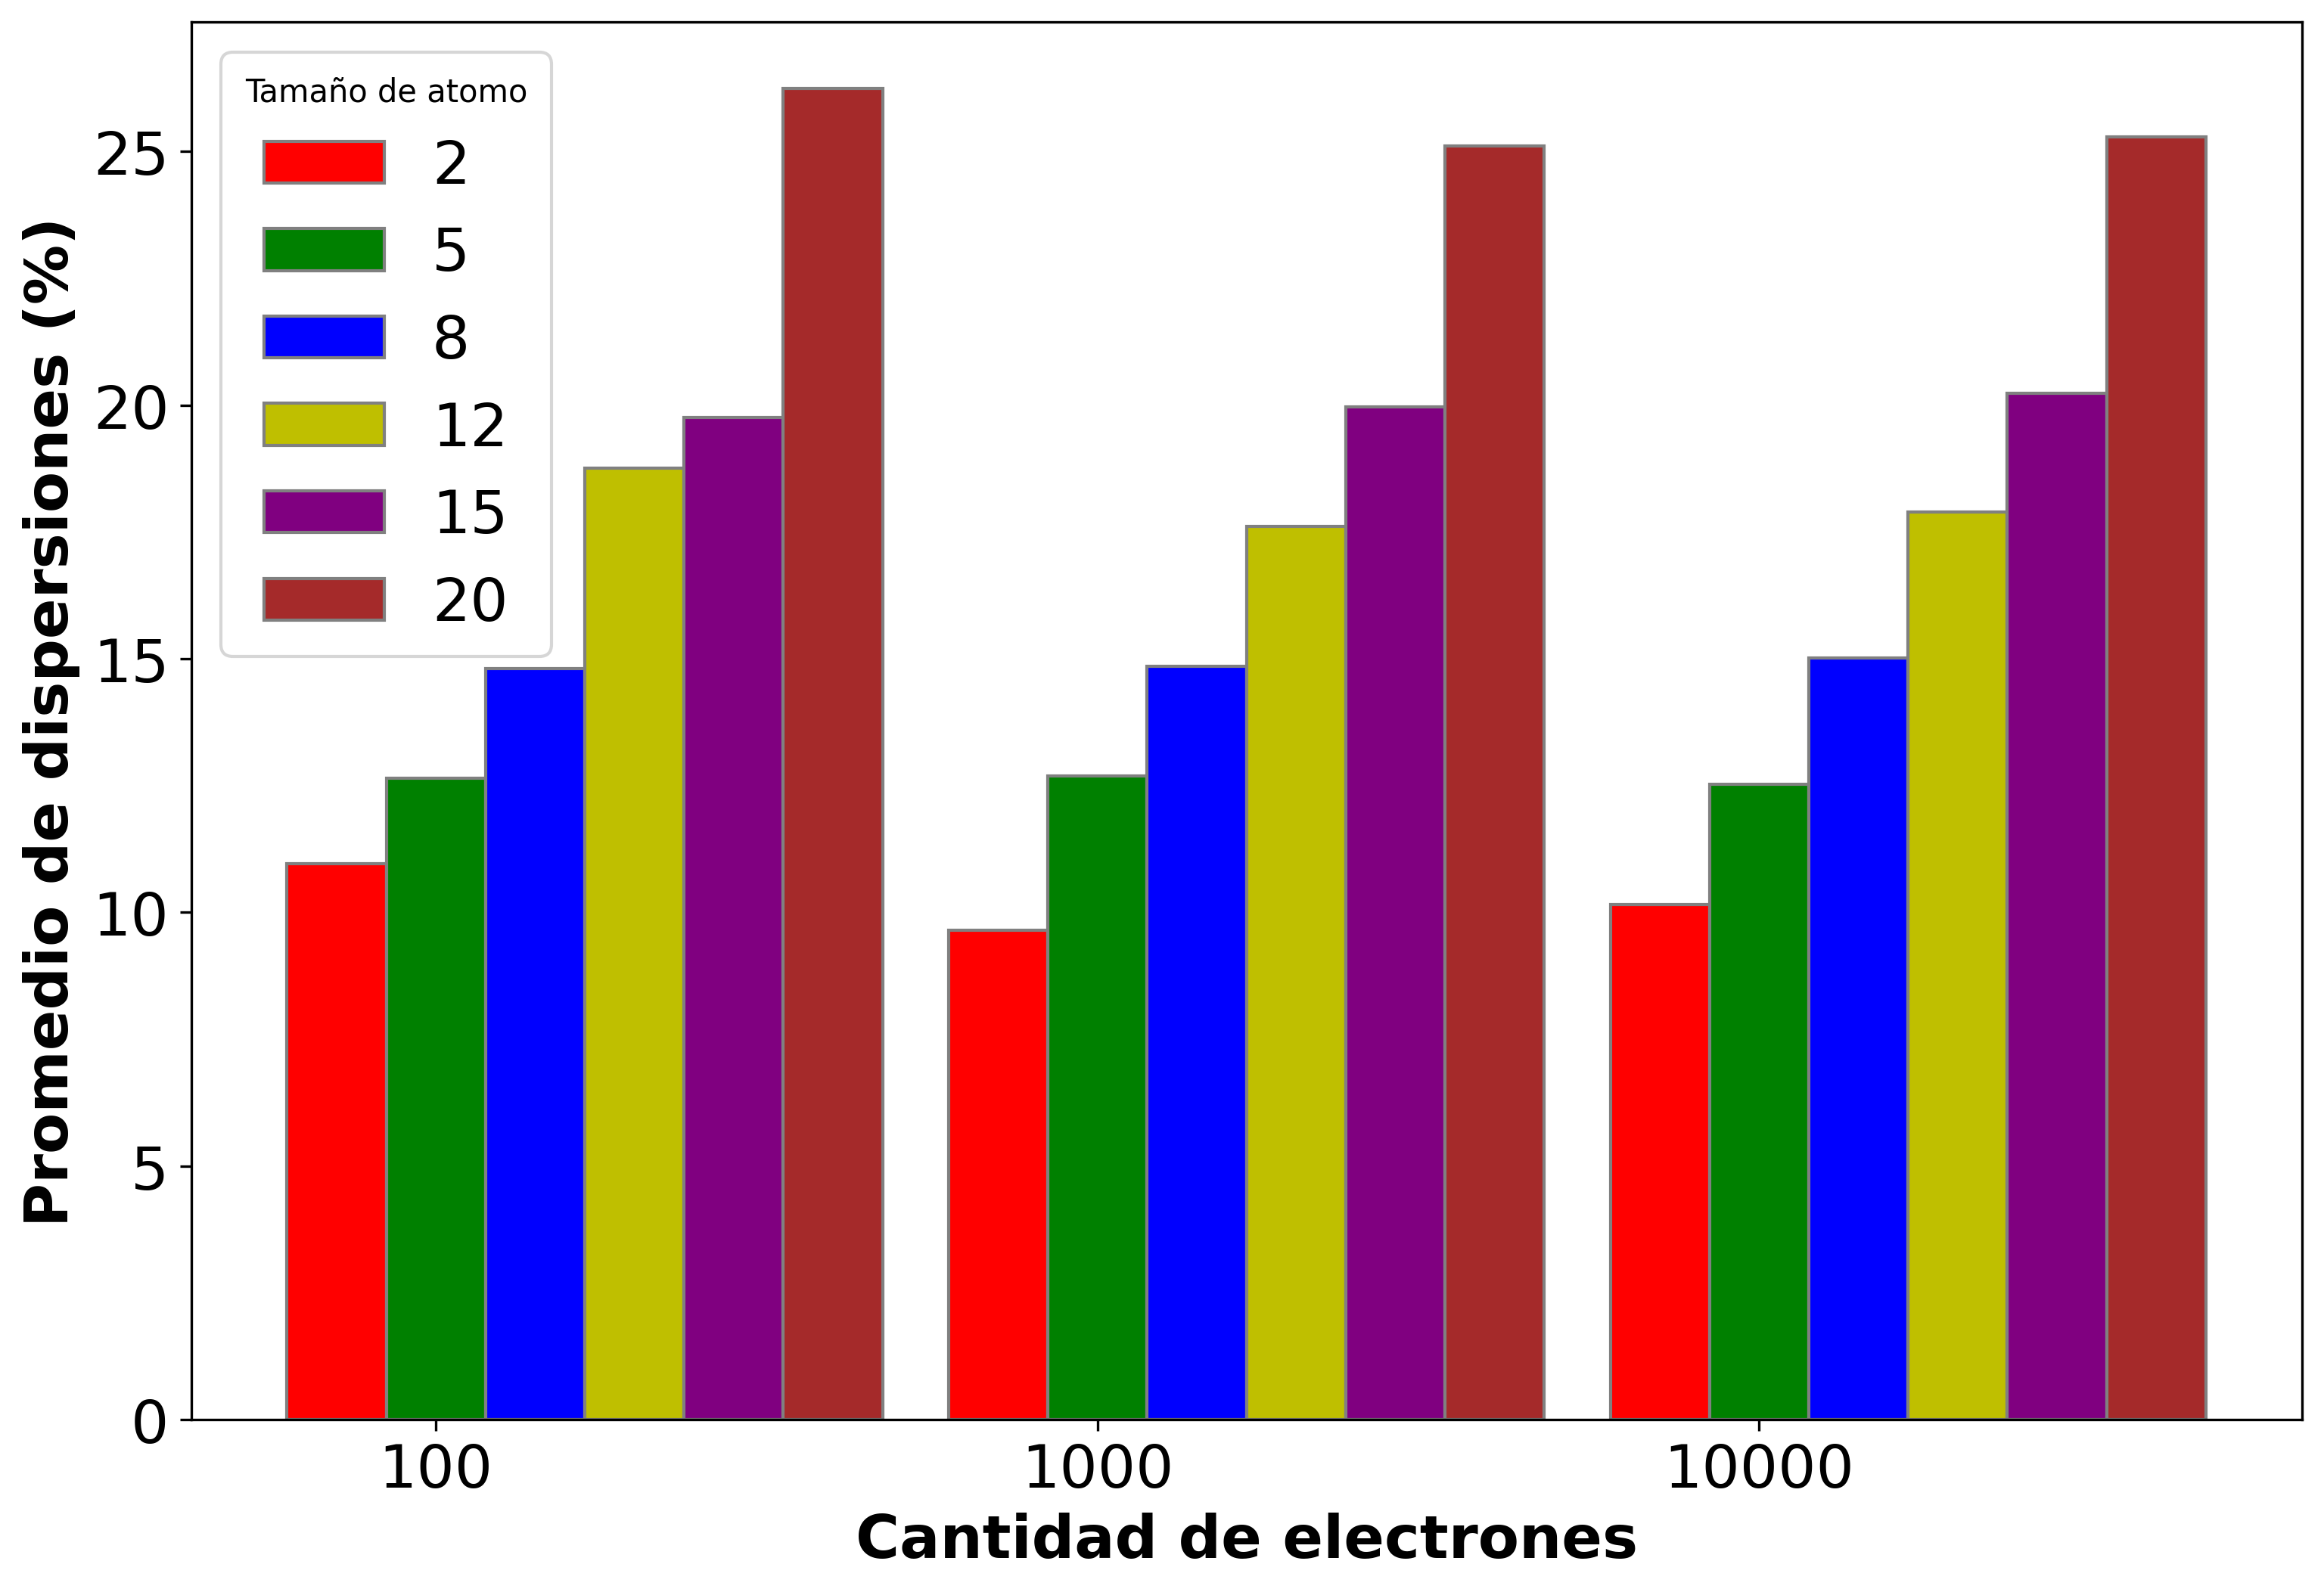
\includegraphics[scale=0.33]{bar_plot.png}
    \caption{Gráfico de promedios de dispersión respecto al tamaño de átomo.}
    \label{barras}
\end{figure}

El porcentaje de dispersiones cambió respecto al tamaño del átomo así como en la cantidad de electrones y dichos resultados pueden ser observados gráficamente en la figura \ref{barras}, 

\begin{table}[h!]
    \centering
    \caption{Tabla de resultados en dispersiones por tamaño de átomos y cantidad de electrones.}
    \begin{tabular}{|c|c|c|}
       \hline
        Cantidad & Tamaño de & Electrones\\
       electrones& átomo & dispersos (\%) \\
       \hline
       & 2 & 10.96 \\
       & 5 & 12.64 \\
       100& 8 & 14.80 \\
       & 12 & 18.76 \\
       & 15 & 19.76 \\
       & 20 & 26.24 \\
       \hline
       & 2 &9.64\\
       & 5 & 12.68 \\
       1000& 8 & 14.85 \\
       & 12 & 17.61 \\
       & 15 & 19.96 \\
       & 20 & 25.10\\
       \hline
       & 2 & 10.15\\
       & 5 & 12.52\\
       10000& 8 & 15.02 \\
       & 12 & 17.89\\
       & 15 & 20.22\\
       & 20 & 25.28\\
       \hline
    \end{tabular}
    \label{tabla1}
\end{table} 

Los datos extraídos de los gráficos se puede visualizar en la tabla \ref{tabla1} donde se puede hacer una determinación de si a mayor número de electrones es significativo el mejoramiento en el porcentaje de electrones o si depende en su mayoría por el tamaño del átomo.

\subsection{Discusión}
Los resultados que fueron encontrados gráficamente se procesan mediante análisis estadísticos por el método de \texttt{Kruskal Wallis} el cual arroja si las variables utilizadas en el experimento son estadísticamente significativas.

\begin{table}[h!]
    \centering
    \caption{Pruebas estadísticas \texttt{Kruskal Wallis}.}
    \begin{tabular}{|c|c|c|}
       \hline
        Datos & Prueba & Valor\\
       & estadística & P \\
       \hline
       Tamaño de átomo& 0.035 & 0.982 \\
       Cantidad de electrones& 16.578 & 0.005 \\
       \hline
    \end{tabular}
    \label{tabla2}
\end{table} 
De los resultados mostrados en la tabla \ref{tabla2} se pudo concluir que el valor \texttt{p} para el tamaño de átomos fue mayor a 0.05 mientras que para la cantidad de electrones no se cumplió. 

\section{Conclusiones}
Se puede concluir con este trabajo que el efecto de dispersión de electrones depende en gran proporción a la cantidad de electrones que sean impactados para obtener mejor el porcentaje de dispersión así como el tamaño o fuerza del átomo, se observa que entre mayor sea esta fuerza la dispersión es mayor, por lo tanto menos electrones pasan sin sufrir efecto.

Y en base a la prueba estadística se logró concluir que el tamaño del átomo es significativo para la simulación del fenómeno mientras que la cantidad de electrones no resulta ser significativo en el experimento debido a que el valor de \texttt{p} resultó ser menor a $0.05$.

\section{Trabajo a futuro}
Como trabajo a futuro pendiente, la experimentación se puede ampliar a una interacción mas completa donde cada átomo cuenta con nube de electrones que ocasionan fuerzas extra en el electrón incidente, aunado a esto agregar una velocidad al electrón ya que este en la literatura y en la practica se menciona como significativo para el fenómeno.

\bibliographystyle{plainnat}
\bibliography{referencias}

\end{document}